\section{Exponential Backoff}\label{cha:expbackoff}
The technique \textit{exponential backoff} is a method used for reducing interference or collisions. The technique works by incrementing the interval between sending packets which will increase the probability that the packet will get transferred without any other node interference. 

A random interval is needed as the nodes need different intervals. The random interval will improve the chances that one of the sensors will send while the other is waiting. 
Without the random interval the two nodes could collide on the first back off, and both nodes will then back off with the same amount, resulting in another collision. This can keep occurring since the two nodes keeps backing off with the same interval.

\begin{equation}
\label{eq:backoff}
E(c)=2^{c-1}
\end{equation}
The equation used to calculate the maximum backoff interval in milliseconds as stated in equation \ref{eq:backoff}, where $c$ is the current number of collision in transmission between two or more nodes.
There will be added a range from 1 to the calculated maximum backoff, to ensure a range to pick a random number from. Using this equation to calculate the backoff, the delays can be seen in table \ref{cha:expbackoff}.
Figure \ref{fig:expbackoff} shows how exponential backoff is exponentially increasing.

\begin{table}[ht!]
\rowcolors{2}{gray!25}{gray!7}
\centering
\begin{tabular}{ l l l l l }
Attempt                                                                & Back off range                                         & Best case                                       & Average case                                        & Worst case \\ \hline 
\multicolumn{1}{l}{1}                        & \multicolumn{1}{l}{1 to 1}    & \multicolumn{1}{l}{1}  & \multicolumn{1}{l}{1}      & 1          \\
\multicolumn{1}{l}{2}                                                & \multicolumn{1}{l}{1 to 2}                            & \multicolumn{1}{l}{1}                          & \multicolumn{1}{l}{1.5}                            & 2          \\
 
\multicolumn{1}{l}{{3}} & \multicolumn{1}{l}{1 to 4}    & \multicolumn{1}{l}{2}  & \multicolumn{1}{l}{3.5}    & 7          \\
\multicolumn{1}{l}{4}                                                & \multicolumn{1}{l}{1 to 8}                            & \multicolumn{1}{l}{3}                          & \multicolumn{1}{l}{7.5}                            & 15         \\
 
\multicolumn{1}{l}{5}                        & \multicolumn{1}{l}{1 to 16}   & \multicolumn{1}{l}{4}  & \multicolumn{1}{l}{15.5}   & 31         \\
\multicolumn{1}{l}{6}                                                & \multicolumn{1}{l}{1 to 32}                           & \multicolumn{1}{l}{5}                          & \multicolumn{1}{l}{31.5}                           & 63         \\
 
\multicolumn{1}{l}{7}                        & \multicolumn{1}{l}{1 to 64}   & \multicolumn{1}{l}{6}  & \multicolumn{1}{l}{63.5}   & 127        \\
\multicolumn{1}{l}{8}                                                & \multicolumn{1}{l}{1 to 128}                          & \multicolumn{1}{l}{7}                          & \multicolumn{1}{l}{127.5}                          & 255        \\
 
\multicolumn{1}{l}{9}                        & \multicolumn{1}{l}{1 to 256}  & \multicolumn{1}{l}{8}  & \multicolumn{1}{l}{255.5}  & 511        \\
\multicolumn{1}{l}{10}                                               & \multicolumn{1}{l}{1 to 512}                          & \multicolumn{1}{l}{9}                          & \multicolumn{1}{l}{511.5}                          & 1023       \\
 
\multicolumn{1}{l}{11}                       & \multicolumn{1}{l}{1 to 1024} & \multicolumn{1}{l}{10} & \multicolumn{1}{l}{1023.5} & 2047       \\ 
\end{tabular}
\caption{Exponential backoff in milliseconds.}
\label{table:expbackoff}
\end{table}

\begin{figure}[H]
\centering
	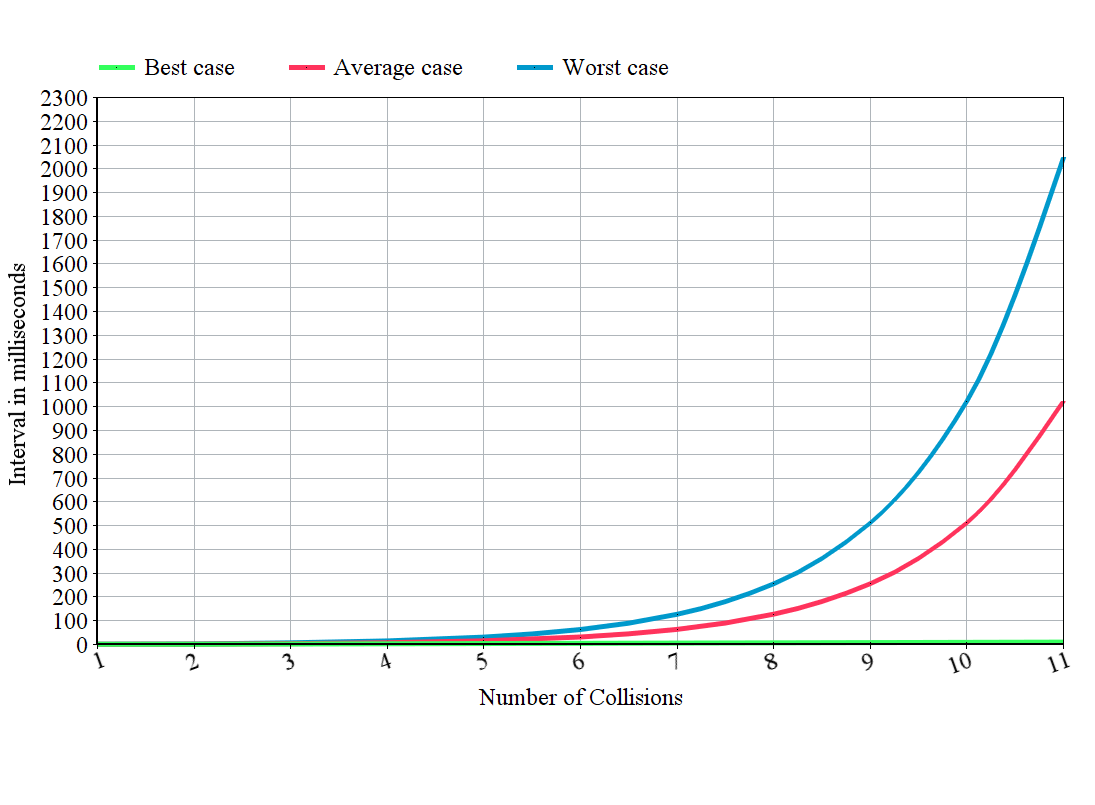
\includegraphics[width=1.0\textwidth]{figures/backoff.PNG}
	\caption{Exponential backoff in milisecounds.}
	\label{fig:expbackoff}
\end{figure}